
\begin{itemize}
	\item Коэффициент аннигилляции $C_AT_{\odot}^2 = 2\Gamma(t = T_{\odot})/C^2$ находится из решения линейного уравнения.
\end{itemize}
\begin{figure}[!h]
	\centering
	\only<1>{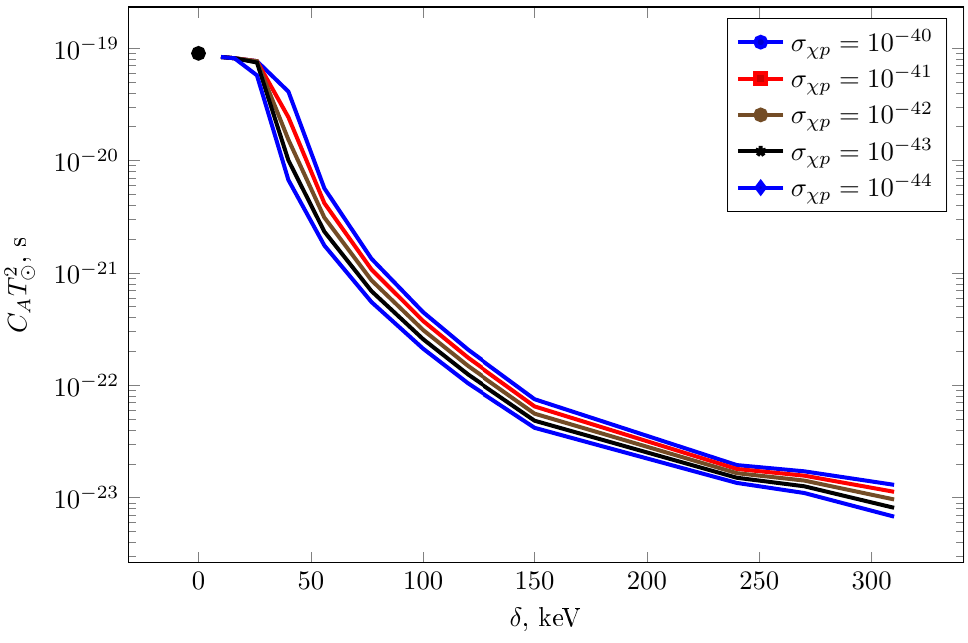
\includegraphics[width=0.7\textwidth]{images/AnnCoeff.png}
	\caption{Коэффициент аннигиляции ТМ $m_{\chi} = 100 \text{GeV}$ ($\chi^*$ --- долгоживущая )}
	}
	\only<2>{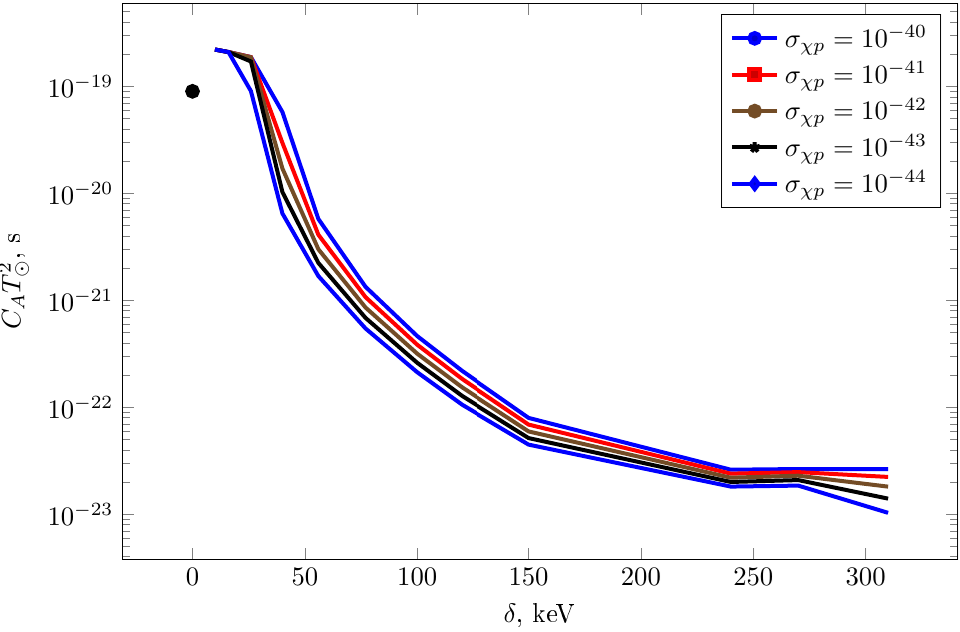
\includegraphics[width=0.7\textwidth]{images/AnnCoeffFD.png}
	\caption{Коэффициент аннигиляции $m_{\chi} = 100 \text{GeV}$ ($\chi^*$ --- короткоживущая )}
	}
\end{figure}